\documentclass[12pt,a4paper]{report}
\usepackage[T1]{fontenc}
%adjust your page margins here
\usepackage[top=0.70in, bottom=0.70in, left=0.8in,right=0.80in]{geometry} % setting the page alignment with this package
\usepackage[pdftex]{graphicx} %for embedding images
\usepackage[%dvips, % commented for pdflatex
bookmarks,  colorlinks=false]{hyperref} %for creating links in the pdf version and other additional pdf attributes, no effect on the printed document
\hypersetup{%
    pdfborder = {0 0 0}
}
\usepackage[final]{pdfpages} %for embedding another pdf, remove if not required
\usepackage{float} %used for figure placement with H as a parameter
\usepackage{hyperref}
\usepackage{pslatex} % for times new roman, old package, but works
\usepackage{array} % for making text bold in table
\usepackage{setspace}
\usepackage{float}
\usepackage{enumerate}
\usepackage{longtable}

\usepackage[font=small,labelfont=bf]{caption}
\def\figurename{\textbf{Figure }}

\usepackage{listings}
\usepackage{color}

\definecolor{dkgreen}{rgb}{0,0.6,0}
\definecolor{gray}{rgb}{0.5,0.5,0.5}
\definecolor{mauve}{rgb}{0.58,0,0.82}
 
\lstset{ %
  language=Java,                % the language of the code
  basicstyle=\footnotesize,           % the size of the fonts that are used for the code
  numbers=left,                   % where to put the line-numbers
  numberstyle=\tiny\color{gray},  % the style that is used for the line-numbers
  stepnumber=1,                   % each line is numbered
  numbersep=5pt,                  % how far the line-numbers are from the code
  backgroundcolor=\color{white},      % choose the background color. You must add \usepackage{color}
  showspaces=false,               % show spaces adding particular underscores
  showstringspaces=false,         % underline spaces within strings
  showtabs=false,                 % show tabs within strings adding particular underscores
  frame=single,                   % adds a frame around the code
  rulecolor=\color{black},        % if not set, the frame-color may be changed on line-breaks within not-black text (e.g. commens (green here))
  tabsize=2,                      % sets default tabsize to 2 spaces
  captionpos=b,                   % sets the caption-position to bottom
  breaklines=true,                % sets automatic line breaking
  breakatwhitespace=false,        % sets if automatic breaks should only happen at whitespace
  title=\lstname,                   % show the filename of files included with \lstinputlisting;
                                  % also try caption instead of title
  keywordstyle=\color{blue},          % keyword style
  commentstyle=\color{dkgreen},       % comment style
  stringstyle=\color{mauve},         % string literal style
  escapeinside={\%*}{*)},            % if you want to add a comment within your code
  morekeywords={*,...}               % if you want to add more keywords to the set
}

%For the header and footer
\usepackage{fancyhdr}
\fancypagestyle{plain}{%
\fancyfoot[L]{\emph{Department of Computer Engineering, SHORT NAME OF COLLEGE, Pune}} % except the center
\fancyfoot[R]{\thepage}
\renewcommand{\headrulewidth}{0.4pt}
\renewcommand{\footrulewidth}{0.4pt}
}

\pagestyle{fancy}

\rhead{\emph{NAME OF PROJECT}}

\fancyfoot[LO,LE]{\emph{Department of Computer Engineering, SHORT NAME OF COLLEGE, Pune}}
\cfoot{}
\fancyfoot[RO, RE]{\thepage}
\renewcommand{\headrulewidth}{0.4pt}
\renewcommand{\footrulewidth}{0.4pt}
%For the header and footer Over

%Page Border
\usepackage{pgf}
\usepackage{pgfpages}

\pgfpagesdeclarelayout{boxed}
{
  \edef\pgfpageoptionborder{0pt}
}
{
  \pgfpagesphysicalpageoptions
  {%
    logical pages=1,%
  }
  \pgfpageslogicalpageoptions{1}
  {
    border code=\pgfsetlinewidth{2pt}\pgfstroke,%
    border shrink=\pgfpageoptionborder,%
    resized width=.95\pgfphysicalwidth,%
    resized height=.95\pgfphysicalheight,%
    center=\pgfpoint{.5\pgfphysicalwidth}{.5\pgfphysicalheight}%
  }%
}
\pgfpagesuselayout{boxed}
\setlength{\parindent}{1cm}
%GLOBAL SETTINGS OVER, DOCUMENT BEGINS
\begin{document}
\renewcommand\bibname{References}
\lhead{ }

%FROM HERE YOUR PAGES START GETTING ADDED

% includes the cover page
\newpage
\begin{center}
\thispagestyle{empty}

\Large{\textbf{A PROJECT REPORT\\ \large{ON}}}\\[0.7cm]
\LARGE{\textsc {\textbf{WORKING WITH DJANGO FORMS}}}\\[0.5cm]
\vspace{0.5cm}
\Large{\textbf{\\Submitted to}}
\LARGE{\textbf{\\SSN College of Engineering\\}}
\vspace{1cm}
\Large{\textbf{\\BY}}\\[0.5cm]
\begin{table}[h]
\centering
\Large{
\begin{tabular}{>{\bfseries}lc>{\bfseries}r}
SUBALAKSHMI SHANTHOSI S & & 186001008 \\
\end{tabular}}
\end{table}
\vspace{0.5cm}
\large{\textbf{UNDER THE GUIDANCE OF}}\\
\large{\textbf{DR. R.S MILTON}}\\
\vspace{1cm}
\large{\textbf{DEPARTMENT OF COMPUTER SCIENCE AND ENGINEERING}}\\
\Large{\textbf{SSN COLLEGE OF ENGINEERING}}\\
\vspace{0.5cm}
\large{\textbf{Rajiv Gandhi Salai (OMR),Kalavakkam -- 603 110 }}
\large{\textbf{\\MAY-2019}}\\
\vspace{1cm}
\Large{\textbf{Sri Sivasubramaniya Nadar College of Engineering(SSNCE)\\}}
(An Autonomous Institution, Affiliated to Anna University, Chennai)\\
\newpage
\end{center}
\newpage

\newpage
\begin{center}
\vspace{5cm}
\thispagestyle{empty}
{\fontfamily{ptm}\selectfont
\Large{\textsc {\textbf{WORKING WITH DJANGO FORMS}}}}\\
\Large{\textbf{\\A PROJECT REPORT\\ ON}} \\[0.3cm]
{\fontfamily{ptm}\selectfont
\Large{\textsc {\textbf{WORKING WITH DJANGO FORMS}}}}\\

\Large{\textit{\textbf{\\Submitted by}}}

\vspace{1cm}
\begin{table}[h]
	\centering
	\Large{
		\begin{tabular}{>{\bfseries}lc>{\bfseries}r}
			SUBALAKSHMI SHANTHOSI S & & 186001008 \\
	\end{tabular}}
\end{table}
\vspace{0.5cm}
{\fontfamily{ptm}\selectfont
\large{\textbf{DEPARTMENT OF COMPUTER SCIENCE AND ENGINEERING}}}\\
\vspace*{0.5cm}
\Large{\textbf{SSN COLLEGE OF ENGINEERING}}\\
\large{\textbf{\\MAY-2019}}\\
\vspace{10cm}


\includegraphics[scale=0.35]{ssnLogoNew.png}

\Large{\textbf{Sri Sivasubramaniya Nadar College of Engineering\\}}
{(An Autonomous Institution, Affiliated to Anna University, Chennai)}\\
\end{center}
\newpage

% includes the certificate page
\begin{center}
\thispagestyle{empty}
\vspace{10cm}
\LARGE{\textbf{Sri Sivasubramaniya Nadar College of Engineering }} \\ 
\normalsize{(An Autonomous Institution, Affiliated to Anna University, Chennai)} \\
Rajiv Gandhi Salai (OMR), Kalavakkam - 603 110 \\
\vspace{2cm}

{\Huge \textbf{BONAFIDE CERTIFICATE }}\\[0.5cm]
\end{center}
\linespread{1.13}
\large{\centering{Certified \space  that \space this \space project\space report \space  titled,}
\textbf{...{``WORKING WITH DJANGO FORMS``}} \space is \space the \space bonafide \space work \space of \space \textbf{''SUBALAKSHMI SHANTHOSI S(186001008)....''} \space who carried out the project work under my
guidance. }\\[0.2cm]
\begin{spacing}{0}
\vspace{3.0cm}
\large{\textbf{SIGNATURE:}}\hspace*{2.5in}\large{\textbf{SIGNATURE:}}\\
\vspace*{1,5cm}

\hspace*{0.02in}\textbf{HEAD OF THE DEPARTMENT}\hspace*{0.85in}\textbf{SUPERVISOR}\\[2cm]
\vspace*{1,4cm}
Submitted for end semester project examination held on ........................\\[8cm]

\textbf{INTERNAL EXAMINER }
\end{spacing}
 
\newpage

% includes the acknowledgements page
\begin{center}
\thispagestyle{empty}
\LARGE{\textbf{Acknowledgements}}\\[1cm]
\end{center}
\linespread{1.13}
\large{\paragraph{}We are profoundly grateful to \textbf{Prof. GUIDE NAME} for his expert guidance
and continuous encouragement throughout to see that this project rights its
target since its commencement to its completion.}
\large{\paragraph{}We would like to express deepest appreciation towards \textbf{Dr. PRINCIPAL NAME},
Principal, NAME OF COLLEGE, \textbf{Prof. HOD NAME}, 
Head of Department of Computer Engineering and \textbf{Prof. PROJECT COORDINATOR NAME}, Project Coordinator whose
invaluable guidance supported us in completing this project.}
\large{\paragraph{}At last we must express our sincere heartfelt gratitude to all the staff members
of Computer Engineering Department who helped me directly or indirectly during this course of work.}
\begin{flushright}
{
GROUP MEMBER A\\
GROUP MEMBER B\\
GROUP MEMBER C\\
GROUP MEMBER D
}
\end{flushright}
\newpage
 
\newpage

\begin{center}
\thispagestyle{empty}
\vspace{2cm}

\LARGE{\textbf{ABSTRACT}}\\[1.0cm]

\end{center}
\thispagestyle{empty}
\large{\paragraph{} Working with django for designing customisable forms.\\
We begin by designing a basic form with primitive fields with in-build validation suite.Followed by creation of form it is been circulated to all the intended audience for filling whose responses are collected and stored in backstore.}
\large{\paragraph{}The user responses are presented to the creator of the form for viewing and filtering with specific requirements.}\\
\large{\paragraph{} Django functionality of building the \textbf{Model, Template and View (MTV) }} for ensuring separation of concern and enhanced useability in the development process. \\
Django's form functionality can simplify and automate vast portions of this work, and can also do it more securely than most programmers would be able to do in code they wrote themselves.\\

Django handles three distinct parts of the work involved in forms:\\
\begin{itemize}
	\item Preparing and restructuring data to make it ready for rendering.
	\item Creating HTML forms for the data.
	\item Receiving and Processing submitted forms and data from the client.
\end{itemize}
Django model describes the logical structure of an object, its behavior, and the way its parts are represented to us, a \textbf{Form} class describes a form and determines how it works and appears.\\

\vspace*{3cm}
\textbf{Keywords: }Form Design, Django-Form,Django Form Builder % adds the Research Methodology page
\newpage

%TABLE OF CONTENTS AND LIST OF FIGURES ARE AUTOMATICALLY ADDED BY FOLLOWING COMMANDS
%ADD FIGURE OF TABLES IF YOU NEED TO, CHECK DOCUMENTATION
\pagenumbering{roman} %numbering before main content starts


%To reset the Header & Footer for TOC and LOF
\pagestyle{empty}
\addtocontents{toc}{\protect\thispagestyle{empty}}
\tableofcontents % adds Index Page

\addtocontents{lof}{\protect\thispagestyle{empty}}
\listoffigures % adds List of Figures
\cleardoublepage

%And reset back the settings we choose for Header and Footer
\pagestyle{fancy}

\newpage
\pagenumbering{arabic} %reset numbering to normal for the main content

\chapter{Introduction}
\section{SECTION NAME}
\subsection{SUBSECTION NAME 1}
\paragraph{}WRITE HERE

\begin{figure}[H]
  \centering
    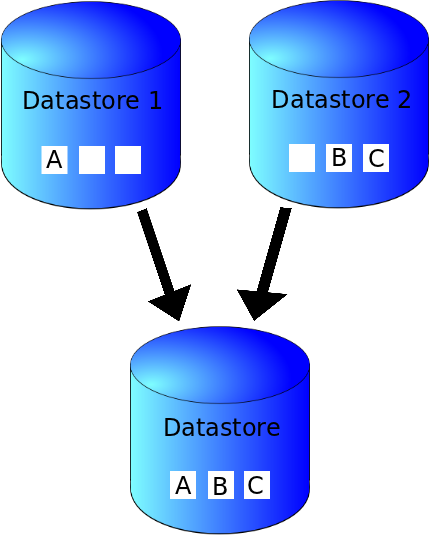
\includegraphics[height= 10cm, width=15cm]{project/images/data-sync}
  \caption{\textbf{IMAGE CAPTION}}
\end{figure}

\subsection{SUBSECTION NAME 2}
\paragraph{}WRITE HERE
 % adds the introduction page
\chapter{Literature Survey}
\section{SECTION NAME}
\paragraph{}WRITE HERE
\begin{enumerate}[a. ]
 \item ITEM 1
 \item ITEM 2
 \item ITEM 3
\end{enumerate} % adds the Literature Survey page
\chapter{Software Requirements Specification}
\section{SECTION NAME}
\subsection{SUBSECTION NAME}
\paragraph{} WRITE HERE.
\chapter{Requirement Analysis}
\section{SECTION NAME}
\paragraph{} WRITE HERE.
\chapter{System Design}
\section{SECTION NAME}
\paragraph{} WRITE HERE.
\chapter{System Testing}
\paragraph{} WRITE HERE.
\section{Test Cases and Test Results}
\begin{longtable}{ | p{1cm} | p{3.5cm} | p{4cm} | p{4cm} | p{4cm} |}
      \hline
      \textbf{Test ID} & \textbf{Test Case Title} & \textbf{Test Condition} & \textbf{System Behavior} & \textbf{Expected Result}\\
      \hline
      T01 & AAAA & BBBB & CCCC & DDDD\\
      \hline
      T02 & AAAA & BBBB & CCCC & DDDD\\
      \hline
      T03 & AAAA & BBBB & CCCC & DDDD\\
      \hline
\end{longtable}

\textbf{Note: Testing should be performed manually}
\chapter{Project Planning}
\section{SECTION 1}
\paragraph{} WRITE HERE.

\chapter{Implementation}
\paragraph{}WRITE HERE, PARAGRAPH 1.
\paragraph{}WRITE HERE, PARAGRAPH 2.

\begin{figure}[H]
  \centering
    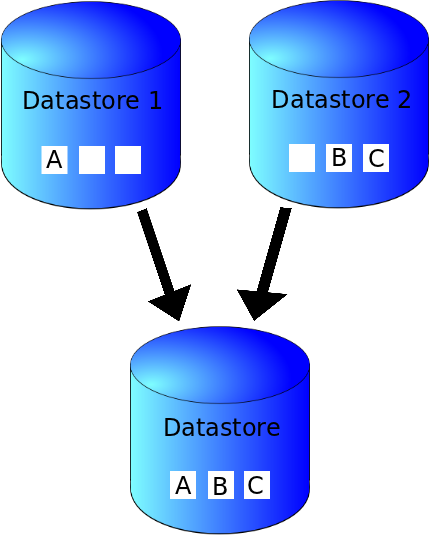
\includegraphics[scale=0.5]{project/images/data-sync}
  \caption{\textbf{IMAGE CAPTION}}
\end{figure}

\begin{lstlisting}
  PASTE YOUR CODE HERE
\end{lstlisting}
\newpage

 % adds the Project Design
\chapter{Screenshots of Project}
\section{SECTION NAME}
\vspace{2cm}
\begin{figure}[H]
  \centering
    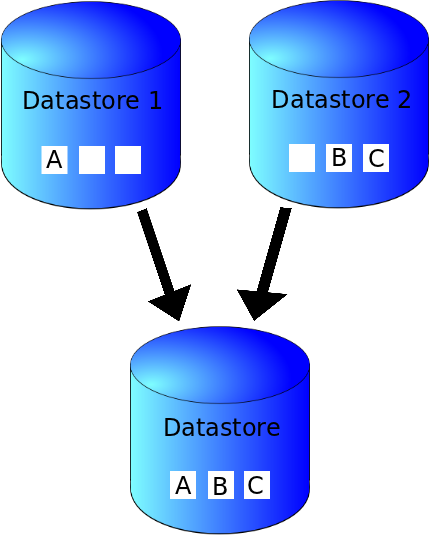
\includegraphics[height= 11cm, width=17cm]{project/images/data-sync}
\end{figure}
\newpage
\begin{figure}[H]
  \centering
    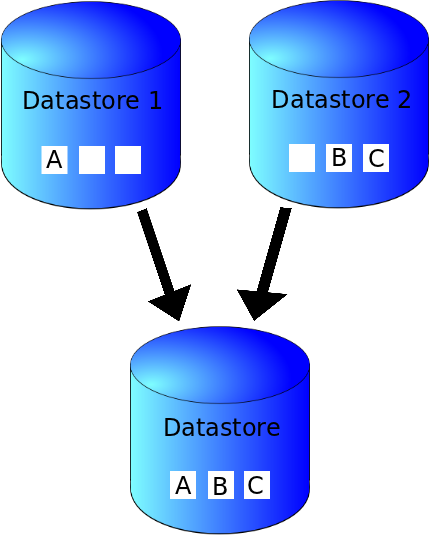
\includegraphics[height= 11cm, width=17cm]{project/images/data-sync}
\end{figure}
\vspace{1cm}
\begin{figure}[H]
  \centering
    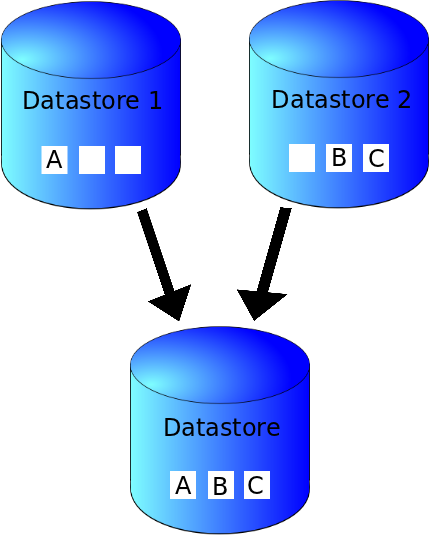
\includegraphics[height= 11cm, width=17cm]{project/images/data-sync}
\end{figure}
\chapter{Conclusion and Future Scope}
\section{Conclusion}
\paragraph{}WRITE HERE.
\section{Future Scope}
\paragraph{}WRITE HERE.
\begin{itemize}
 \item ITEM 1
 \item ITEM 2
 \item ITEM 3
\end{itemize} % adds the Scheduling and Planning page
\addcontentsline{toc}{chapter}{References}
\begin{thebibliography}{99}
\bibitem{WRITE A SHORT-NAME WITHOUT SPACE} \emph{NAME OF IEEE PAPER}; NAME OF AUTHORS
\bibitem{WRITE A SHORT-NAME WITHOUT SPACE} \url{http://EXAMPLE.com}
\end{thebibliography} % adds the References page

\end{document}